\documentclass[
	ngerman,
	ruledheaders=section,%Ebene bis zu der die Überschriften mit Linien abgetrennt werden, vgl. DEMO-TUDaPub
	class=report,% Basisdokumentenklasse. Wählt die Korrespondierende KOMA-Script Klasse
	thesis={type=master},% Dokumententyp Thesis, für Dissertationen siehe die Demo-Datei DEMO-TUDaPhd
	accentcolor=3c,% Auswahl der Akzentfarbe
	custommargins=false,% Ränder werden mithilfe von typearea automatisch berechnet
	marginpar=false,% Kopfzeile und Fußzeile erstrecken sich nicht über die Randnotizspalte
	%BCOR=5mm,%Bindekorrektur, falls notwendig
	parskip=half-,%Absatzkennzeichnung durch Abstand vgl. KOMA-Sript
	fontsize=11pt,%Basisschriftgröße laut Corporate Design ist mit 9pt häufig zu klein
%	logofile=example-image, %Falls die Logo Dateien nicht vorliegen
	IMRAD=false,%Abschalten von IMRAD-Warnings wegen fehlender Labels
]{tudapub}

\usepackage[acronym,nonumberlist,nopostdot,shortcuts]{glossaries}
\usepackage{multicol}
\usepackage{url}
\usepackage{graphicx}
\usepackage{tikz}
\usepackage{graphicx}
\usepackage{xfrac}
%\usepackage{amssymb}
\usepackage{epstopdf} 
\usepackage{eurosym}
%\usepackage{lmodern} % nicht nutzen dies schaltet die TU Schriftart aus!!!!!!!!!
\usepackage{booktabs} % hübschere Tabellen als der LaTeX-Standard
\usepackage{amsmath}
\usepackage{placeins}
\usepackage{siunitx}
\usepackage{multirow}
\usepackage{adjustbox}
\usepackage{mwe}
\usepackage{algorithm}
\usepackage{algpseudocode}

\algnewcommand\algorithmicforeach{\textbf{for each}}
\algdef{S}[FOR]{ForEach}[1]{\algorithmicforeach\ #1\ \algorithmicdo}

%\usepackage{subfig}
\usepackage{paralist}
% Der folgende Block ist nur bei pdfTeX auf Versionen vor April 2018 notwendig
\usepackage{iftex}
\ifPDFTeX
\usepackage[utf8]{inputenc}%kompatibilität mit TeX Versionen vor April 2018
\fi

%%%%%%%%%%%%%%%%%%%
%Sprachanpassung & Verbesserte Trennregeln
%%%%%%%%%%%%%%%%%%%
\usepackage[english, main=english]{babel}
\usepackage[autostyle]{csquotes}% Anführungszeichen vereinfacht
\usepackage{microtype}


%%%%%%%%%%%%%%%%%%%
%Literaturverzeichnis
%%%%%%%%%%%%%%%%%%%
\usepackage{biblatex}   % Literaturverzeichnis
%\bibliography{DEMO-TUDaBibliography}


%%%%%%%%%%%%%%%%%%%
%Tabellen
%%%%%%%%%%%%%%%%%%%
%\usepackage{array}     % Basispaket für Tabellenkonfiguration, wird von den folgenden automatisch geladen
\usepackage{tabularx}   % Tabellen, die sich automatisch der Breite anpassen
%\usepackage{longtable} % Mehrseitige Tabellen
%\usepackage{xltabular} % Mehrseitige Tabellen mit anpassarer Breite
\usepackage{booktabs}   % Verbesserte Möglichkeiten für Tabellenlayout über horizontale Linien

%%%%%%%%%%%%%%%%%%%
%Paketvorschläge Mathematik
%%%%%%%%%%%%%%%%%%%
\usepackage{mathtools} % erweiterte Fassung von amsmath
\usepackage{amssymb}   % erweiterter Zeichensatz
\usepackage{siunitx}   % Einheiten

%%%%%%%%%%%%%%%%%%%
%Eigene Importe
%%%%%%%%%%%%%%%%%%%
\usepackage{amssymb}% http://ctan.org/pkg/amssymb
\usepackage{pifont}% http://ctan.org/pkg/pifont
\newcommand{\cmark}{\ding{51}}%
\newcommand{\xmark}{\ding{55}}%
\usepackage{svg}

%Formatierungen für Beispiele in diesem Dokument. Im Allgemeinen nicht notwendig!
\let\file\texttt
\let\code\texttt

\usepackage{pifont}% Zapf-Dingbats Symbole
\newcommand*{\FeatureTrue}{\ding{52}}
\newcommand*{\FeatureFalse}{\ding{56}}
%\bibliographystyle{IEEEtran}

\usepackage{subcaption}
\usepackage{graphicx}
\newcommand*{\mrm}[1]{\ensuremath{\mathrm{#1}}}

\usepackage{listings}
\definecolor{eclipseStrings}{RGB}{42,0.0,255}
\definecolor{eclipseKeywords}{RGB}{127,0,85}
\colorlet{numb}{magenta!60!black}

\lstdefinelanguage{json}{
    basicstyle=\normalfont\ttfamily,
    commentstyle=\color{eclipseStrings}, % style of comment
    stringstyle=\color{eclipseKeywords}, % style of strings
    numbers=left,
    numberstyle=\scriptsize,
    stepnumber=1,
    numbersep=8pt,
    showstringspaces=false,
    breaklines=true,
    frame=lines,
    backgroundcolor=\color{white}, %only if you like
    literate=
        *{0}{{{\color{numb}0}}}{1}
         {1}{{{\color{numb}1}}}{1}
         {2}{{{\color{numb}2}}}{1}
         {3}{{{\color{numb}3}}}{1}
         {4}{{{\color{numb}4}}}{1}
         {5}{{{\color{numb}5}}}{1}
         {6}{{{\color{numb}6}}}{1}
         {7}{{{\color{numb}7}}}{1}
         {8}{{{\color{numb}8}}}{1}
         {9}{{{\color{numb}9}}}{1}
}


\bibliography{bib/Literatur}
%Own Commands

\linespread{1.25}

\begin{document}

\Metadata{
	title=Modeling and Analysis of Human Behavior Impacts on Energy Systems during Crisis Events,
	author=Isabella Nunes Grieser
}

\title{Modeling and Analysis of Human Behavior Impacts on 
Energy Systems during Crisis Events}
\subtitle{Modellierung und Analyse der Auswirkung des menschlichen
Verhaltens auf Energienetze während Krisensituationen}
\author[Isabella Nunes Grieser]{Isabella Nunes Grieser}%optionales Argument ist die Signatur, 
%\birthplace{Geburtsort}%Geburtsort, bei Dissertationen zwingend notwendig
\reviewer{Prof. Dr. Florian Steinke \and M.Sc. Tobias Gebhard}%Gutachter
\publishers{}
%Diese Felder erden untereinander auf der Titelseite platziert. 
%\department ist eine notwendige Angabe, siehe auch dem Abschnitt `Abweichung von den Vorgaben für die Titelseite'
\department{etit} % Das Kürzel wird automatisch ersetzt und als Studienfach gewählt, siehe Liste der Kürzel im Dokument.
\institute{\includegraphics*[width=4cm]{gfx/EINS_Logo}}
\group{}

\submissiondate{\today}
\examdate{\today}

%	\tuprints{urn=1234,printid=12345}
%	\dedication{Für alle, die \TeX{} nutzen.}

\maketitle
\affidavit

\begin{abstract}[english]


Multiple examples have shown how vulnerable supply 
chains are to unexpected changes in consumer demand in recent history.
Information on social media may be the cause of changes in demand by 
influencing consumers to panic buy certain goods.
Until now, these events primarily involved physical goods.
However, critical infrastructure that deals with non-physical 
goods such as the power grid could also be affected by 
sudden spikes of consumer demand. Critical infrastructure
needs to be resilient towards various kinds of threats, hence it 
is important to analyze possible threats to the infrastructure
before they happen to prepare countermeasures.
In this thesis, the effects of demand changes based on information
which is being spread are modelled and analyzed with different scenarios. 
A simulation framework is implemented, with a graph-based social network model 
and a epidemological model based on the 
susceptible-infectious-recovered model (SIR) to 
model information propagation processes. 
Furthermore, information propagation parameters 
are estimated with social media data. 
Then, four theoretical scenarios are used as examples
to analyze sudden changes in demand for the power grid.
The analysis shows that simultaneous shifts 
in consumer demand could pose risks to the 
stability of the power grid. 
Additionally, further adoption of 
energy-intensive technologies 
such as electric vehicles 
are shown to amplify the impact of 
synchronized changes in consumer 
demand on the energy infrastructure.


\end{abstract}
% \begin{abstract}[ngerman]

\end{abstract}

\tableofcontents


%\listoftables
%\listoffigures
\printglossary %[type = \acronymtype]

\chapter{Introduction}

This Chapter aims to show the significance of information and 
the subsequent human action based on it
in the context of the power grid infrastructure.
Furthermore, the necessity to understand the possible consequences 
of human behavior on critical infrastructure is shown. 
First, in Section \ref{contextmotivation}, the necessary context and 
motivation for this Thesis is provided.
Then, the problem that is considered in this thesis is described 
in Section \ref{problemstatement}. Afterward, the contribution that this
Thesis proposes is presented in Section \ref{contribution}, 
followed by the outline of this work in Section \ref{outline}.

\section{Context and Motivation}
\label{contextmotivation}

During the COVID-19 pandemic, drastic changes in consumer behavior
lead to massive supply issues, thus showing how sensitive supply markets 
can be to changes in consumer demand.
For this reason, research in how changes in demand during crisis occur
started to gain interest. One reason for changes in consumer demand is 
social media usage. Through social media, consumers can gain new information
and change their demand on certain goods based on the information received 
through these channels \cite{naeem2021social}.
The research for these drastic changes in consumer demand are usually
done for regular, physical goods. But the results shown in these 
works may not translate well to critical infrastructure
with other characteristics as physical goods such as 
water, energy or communications systems.

One critical infrastructure that is specially important for 
our society is the power grid infrastructure.
There are no examples of drastic changes in consumer behavior leading
based on information on social media leading to supply issues or
even the breakdown of the power grid in real life. Nonetheless, there 
are still possible events that could happen where the demand for
electricity may increase due to information on social media.
For example, a false notice of reduced prices for electricity
during peak demand hours may lead to increased demand during 
a time where the demand is already high. The additional demand
may increase the total demand to a level that the power grid
cannot support, thus leading to blackouts.
Another example would be that coordinated actions to reduce
energy, either in regards to combat climate change \cite{earthday}
or as a means of an attack against the state by conspiracy theorists,
lead to a non-negligible mismatch of supply and demand.


\section{Problem Statement}
\label{problemstatement}

To reduce the probability of blackouts, 
the resilience of the power grid is of vital importance.
To assure the resilience of the power grid, a variety of possible 
scenarios which could negatively affect the power grid need
to be analysed and countermeasures need to be made for all possible scenarios.
Thus, it is reasonable to analyse theoretical scenarios that, even though
they never happened until the present time, could plausibly happen. This 
would allow policymakers to draw countermeasures to these possible scenarios
and allow for quick and decisive actions to be taken by relevant 
parties.

Until now, there are already works which analyse the possible effects
of information, specially misinformation, on the power
grid. But these works were of theoretical nature and did not 
propose any kind of detection system to warn of a possible 
for the power grid. Furthermore, these works did only analyse the 
possibility of a false notice of reduced electricity prices.
No other scenarios are analysed in these works. 


\section{Contribution}
\label{contribution}
This Thesis contributes to the problem of power demand changes
through social media in two points.
First, this Thesis analyses multiple different scenarios, in which
information on social media lead to a change in power demand.
These include both the scenario where there is a false notice of 
reduced prices and other scenarios.
Furthermore, this Thesis proposes a framework to predict if 
a certain topic on social media is propagating through social media
in a speed that could lead to issues for the power grid.

\section{Outline}
\label{outline}

First, the necessary background necessary for this Thesis is explained
in Chapter \ref{background}. Chapter \ref{background} includes an introduction
to the concept of panic buying and the relevance of social media 
to this phenomenom in Section \ref{panicbuying}. Then, in 
Section \ref{graphbasics}, the foundations of graphs are introduced,
how they can represent real networks and how graphs can be
generated randomly. Next, in Section \ref{informationdiffsection},
different algorithms to model information propagation in 
social networks are described. Last, in \ref{powerloadsection},
the problem of power load forecasting is explained and 
variables that are connected with human behavior
are introduced. In addition, their correlation with power consumption are 
described.

In Chapter \ref{relatedworks}, the related works of relevance for 
this Thesis are introduced.

Next, in Chapter \ref{implementationall}, the framework to
analyse and predict possible power demand surges based on
information on social media is introduced.
First, the simulator is introduced in Section \ref{modelsocialnetwork}.
Then, in Section \ref{parameterestimationalgo}, 
an algorithm to estimate parameters to realistically simulate
the effects of information on social media is introduced and 
the all steps of the framework are explained.

Then, in Chapter \ref{results}, the different scenarios considered in this
Thesis are analysed. ..... (TODO)
\chapter{Background}
\label{background}

In this chapter, the fundamental concepts necessary to understand 
this Thesis are explained.
First, in Section \ref{panicbuying}, 
the general concept of panic buying,
its consequences and what may lead to panic buying is explained.
Second, in Section \ref{graphbasics}, 
the fundamental theory of graph systems are 
introducted and multiple attributes to describe graphs are defined.
Furthermore, the concept of random graphs and multiple random 
graph algorithms are described.
Third, the concept of information diffusion
and multiple algorithms to model information diffusion are introduced
in Section \ref{informationdiffsection}.
Forth, in Section \ref{powerloadsection}, 
the field of power load forecasting is introduced and 
different human-based variables that 
correlate with the power consumption are described.


\section{Panic Buying as a Result from Social Media Influence}
\label{panicbuying}

Among consumer behaviors that have become increasingly concerning in modern times, 
one that stands out is the phenomenon of panic buying.
It occurs when there is an unusual surge in sales of 
specific goods due to extraordinary situations, such as natural disasters, 
pandemics, or the spread of misinformation among the general population.
Currently, this phenomeon has gained interest since it occured
during the COVID-19 pandemic,
where the demand for disinfectants, soap and toilet paper increased significantly
\cite{covidpanicbuying}. Nonetheless, panic buying is not a new behavior.
There are other historical examples for panic buying behavior.
These include the Spanish Flu
in 1918, where there was an increasing demand for medications 
\cite{honigsbaum2013regulating}. Another example is the Cuban Missile Crisis 
in 1962, where the sales of canned foods increased significantly 
\cite{george2004awaiting}. 
Last, during hurricane Irma in 2017 in the US, the affected population bought
significantly more fuel, bottled water 
and other essential goods in anticipation of the hurricane \cite{irmahurricane},
thus leading to shortages.

There are multiple possible reasons for panic buying behavior. These reasons 
are described in the work of \textit{Prentice et al.}
\cite{prentice2022antecedents}. They include:

\begin{itemize}
    \item Peer Pressure: The knowledge that other people fear shortages and 
    stock-outs leads to people being influenced by their peers' fears and leads
    to them fearing shortages themselves, thus forcing them to also buy excessively.
    \item Sense of Security: Given the uncertainty that the general population
    feels during a crisis, people want to secure their own future. This 
    also applies to situations where people expect 
    shortages due to the fears and actions of their peers.
    Thus, they participate in panic buying to the secure their
    own stockpile.
    \item Media Influence: The stories of shortages on the media
    lead to a distorted view that there exists a shortage, thus increasing 
    the people's fears that a shortage exists or is drawing near and consequently
    leading them to participate in panic buying.
\end{itemize}

One cause of special interest for this thesis is the influence of 
social media on the panic buying phenomenom. 
Multiple reasons for why social media influences consumer demand, 
specifically in the case of the COVID-19 pandemic,
are discussed in the work of \textit{Naeem} \cite{naeem2021social}.
His work showed that since people are spreading their 
own experiences on social media, the messages generated from their peers feel
more personal and lead to a stronger reaction by increasing the will to 
socially distance and stockpiling supplies. Additionally, people are 
influenced more strongly by their friends' posts and advices on social media.
Moreover, since friend circles become more 
internationalized through the global nature of social media networks,
events in other countries and the
possible consequences for one's own country can be analyzed, thus
leading to a reaction. As an example,
shortage of a specific good in one country can lead to people in other countries
assuming that the shortage may happen in one's own country, thus leading to 
panic buying in one's own country. 
The next discovery was that people in positions of authority and with expertise,
such as politicians, organizations, and experts, can use social media to increase 
the outreach of their messages, leading to people talking about their 
recommendations and policies.
Last, it was also proven that social media may increase rumor spreading,
consequently leading to panic buying \cite{naeem2022understanding}.
In conclusion, social media can both amplify the messages and rumors that lead to 
panic buying and it can amplify the messages of governments and organizations 
that may inhibit panic buying.



\section{Graph as a Representation of Social Media Networks}
\label{graphbasics}
Graph are often used to model real-world systems.
A graph is an abstract structure that represents a set of objects and the 
relationship between the objects. 
This Thesis focuses primarily on social media networks
\cite{socialgraphexample}. Nonetheless, graphs can 
also be applied to other real-world systems, such as economic systems 
\cite{economicsgraph} or power grids \cite{powergraphexample}.


Per definition, a graph $G(V, E)$ consists of a set of vertices (or nodes) $V$ and a 
set of edges $E$. Each edge connects two nodes $x, y \in V$ and is 
written as $e=(x, y)$. This means that for all $e\in E$, the 
condition  $e \subseteq\{ (x, y) \mid x, y \in V  \}$ 
is valid.

There are multiple subtypes of graphs. A directional graph is a graph 
whose edges have a source node $a$ and target node $b$, thus representing
a direction from $a$ to $b$. If the edges do not fulfill this 
condition, i.e. if the edges do not show a direction, a graph is unidirectional.
In addition, a graph may have attributes, also called weights, 
associated to its edges. These graphs are called weighted graphs.

There are also multiple metrics that can be calculated in a graph
and that show its characteristics. Relevant metrics are 
explained below \cite{basicnetwork}.
\begin{itemize}
    \item The degree $c_v$ of a node $v \in V$ is the number of edges connected to the
    node $v$. 
    \item The degree distribution $P_k$ is the probability distribution 
    of the node degrees $k$ over all nodes $V$ in the graph $G$
    \item The average path length $l$ is the average number of steps between
    the shortest paths for all possible node combinations in a graph.
    \item The clustering coefficient $C$ describes how densely connected
    the vertices in the graph $G$ are. There are two different types of
    clustering coefficient. The global clustering
    coefficient is calculated as \\
    $C=\frac{(3 \cdot\text{number of triangles})}{(\text{number of connected triples})}$,
    where a connected triple means there are three nodes $a,b,c\in V$ with
    the edges $(a,b), (b,c) \in E$ (and where the edge $(a,c)$ may 
    possibly exist) and the number of triangles mean
    that the three vertices $a,b,c\in V$ that are fully connected to each other.
    The local clustering coefficient is calculated for a single node $i$
    and is defined as $C_i=\frac{\text{number of pairs of neighbors of }i 
    \text{ that are connected to each other}}
    {\text{number of pairs of neighbors of }i }$.
\end{itemize}

Furthermore, graphs that specifically model networks follow two special 
characteristics that may differ from other types of graphs.
First, network models are often scale-free networks.
Scale-free networks are networks that follow the power law distribution.
The law stipulates that the degree distribution $P_k$ of a network
follows the power distribution.
This means that the probability that a node has a certain degree $k$ 
is proportional to the function $k^{-\gamma}$, where
$\gamma>1$.
Moreover, most nodes are not directly connected to one another in a network.
Nonetheless, it is likely that they share the same neighbors or that their
neighbors share the same neighbors. These networks are called small-world 
networks. In these networks, most nodes can reach most other
nodes by a small number of steps. For a network
to be considered a small-world network, its average path length $l$ 
needs to fullfil the condition $l\sim ln(n)$, where $n$ is the number
of nodes in the graph \cite{wattsmodel}.

One network that is of special interest in this thesis are social networks.
Social networks describe how humans are socially connected. 
These networks may model friendship, scientific co-authorship 
or online social media networks, for example \cite{basicnetwork}. 
These kinds of networks can be modeled as graphs, where the nodes 
are the general population modeled in the system
and the edges model the relationship between the 
different people.
Social networks often share similar characteristics. The study of 
\textit{Mislove et al.} that focuses on online social media networks
shows that social networks fulfill the small world characteristic,
have a high clustering coefficient and are scale-free networks
\cite{mislovesocialnetworkcharacteristics}. Thus, to accurately represent 
social networks, a graph should ideally fulfill all three characteristics.

\subsection{Random Graphs}
\label{randomgraphssection}
Graphs do not need to be based on real systems. They can also be generated. 
These randomly generated graphs are called random graphs \cite{randomgraphs}.
Typically, specific attributes in a random graph, such as the number of nodes 
or the number of edges, are predetermined, 
while other features are randomly generated using designated algorithms.

There are a number of algorithms used to generate random graphs.
The most commonly used algorithms are introduced in this Section.

\subsubsection{Erdős–Rényi Model}

The oldest random graph algorithm is the 
Erdős–Rényi (ER) random graph. For this type of random graph model, the
number of nodes $n$ and the probability $p$ that an 
edge exists between two nodes are of fixed value \cite{basicnetwork}. 
To generate an ER random graph, the algorithm goes through 
every possible node combination $a, b$ and it creates an edge 
$(a, b)$ given the probability $p$. 
Thus, the number of edges $|E|$ is not fixed.

The characteristics besides the number of nodes and the
probability of the ER graph are generally not known.
Nonetheless, the average value of the other
characteristics to analyze the random graph algorithm can be calculated.
The graph characteristics of this type of random graph are shown in Table 
\ref{erdos-model}.
An important observation is that 
the average degree distribution $P_k$ follows the Poisson distribution
$P_\lambda (k) = \frac{\lambda^k}{k!}\, \mathrm{e}^{-\lambda}$ and
not the power distribution. Thus,
ER graphs do not fulfill the power law characteristic and are consequently
not scale-free. 

\begin{table}[ht!]
    \centering
    \begin{tabular}{|c | c |} 
     \hline
     Mean Number of Edges & 
     $\overline{|E|} = \binom{n}{2}p$  \\ 
     \hline
     Mean Degree & 
     $\overline{c} = (n-1)p$ \\ 
     \hline
     Degree Distribution & 
     $P_k = \frac{\overline{c}^k}{k!} e^{-\overline{c}}$ \\ 
     \hline
     Clustering Coefficient & 
     $C=\frac{\overline{c}}{n-1}=p$ \\ 
     \hline
     Average Path Length \cite{averagepath}& 
     $l = \frac{\ln{n} - \gamma}{\ln(\overline{c}))} + \frac{1}{2}, 
     \gamma=0.57722$ \\ 
     \hline
    \end{tabular}
    \caption{Mean characteristics of the ER random graph \cite{basicnetwork}}
    \label{erdos-model}
\end{table}

\subsubsection{Barabási–Albert Model}

Another well known random graph algorithm is the Barabási–Albert (BA) model 
\cite{barabasimodel}. 
This type of model uses the concept of preferential attachement.
To generate a graph based on this concept, first a small \glqq core\grqq{}
graph with $a$ nodes is created, where $a\ll n$ and $n$ is the final amount of nodes.
Then, $n-a$ nodes are sequentially added to the graph.
These nodes have a higher 
probability to connect to vertices that are already well-connected. 
Thus, the probability $p_i$ that a new node forms an edge with an
existing node $i$ depends on its degree $c_i$. Therefore, the
probability can be calculated as $p_i= \frac{c_i}{\sum_{k}c_k}$.
This concept of preferential attachement leads to the degree distribution
$P_k\sim k^{-3}$. This means that the BA graph 
fulfills the power law characteristic.
This can be seen in the graph characteristics of the random graph
in Table \ref{ba-model}. For this Table, $n$ is defined as the number
of nodes and $m$ as the number of edges that a node
will create when being added to the random graph.

\begin{table}[ht!]
    \centering
    \begin{tabular}{|c | c |} 
     \hline
     Degree & $c\geq m$ \\ 
     \hline
     Degree Distribution & 
     $P_k = \frac{2c_k(c_k+1)}{k(k+1)(k+2)}$ \\ 
     \hline
     Clustering Coefficient \cite{ba_cluster_coeff} & 
     $C=\frac{m}{8}\frac{ln(n)^2}{n}$ \\ 
     \hline
     Average Path Length \cite{averagepath}& 
     $l = \frac{\ln{n}- \ln{m/2} - 1 - \gamma}{\ln(\ln(n))+\ln{(m/2)}} + \frac{3}{2}, 
     \gamma=0.57722$ \\ 
     \hline
    \end{tabular}
    \caption{Mean characteristics of the BA random graph \cite{basicnetwork}}
    \label{ba-model}
\end{table}

\subsubsection{Watts–Strogatz Model}
The last random graph algorithm mentioned in this Section 
is the Watts–Strogatz (WS) random graph \cite{wattsmodel}.
Contrary to BA random graphs, the focus of the WS graph is not to 
form graphs based on the power law, but to create graphs
that follow the small world characteristic more realistically.

The WS random graph model starts with a ring lattice graph, a graph 
with $n$ nodes where each node has the same degree $c$ and 
is connected to its $c$ nearest neighbors. Then, each edge $(a, b)$
may be rewired given the probability $p$, thus reconnecting the edge to  $(a, b')$
instead and creating a shortcut between the two non-neighboring nodes.
Furthermore, the new edge may only be created as long as it does not create
a loop $(a, a)$ and as the link $(a, b')$ does not already exist.
Another version of this algorithm does not rewire existing edges,
but creates new random edges as shortcuts given the probability $p$.
The second version creates a graph that can be considered more 
\glqq random\grqq{} as the graph generated in the first algorithm and is
thus favored over the former algorithm \cite{basicnetwork}.

The graph characteristics of the model can be seen
in Table \ref{ws-model}. Given the degree distribution $P_k$, it can be seen
that the graph does not fulfill the power law characteristic
since it is more similar
to the Poisson distribution than a power distribution. Thus, the WS model
is not scale-free.

\begin{table}[ht!]
    \centering
    \begin{tabular}{|c | c |} 
     \hline
     Degree Distribution & 
     $P_k = e^{-cp}\frac{(cp)^{k-c}}{(k-c)!}$ \\ 
     \hline
     Clustering Coefficient & 
     $C=\frac{3(c-2)}{4(c-1) + 8cp +4cp^2}$ \\ 
     \hline
     Average Path Length & $l = \frac{ln(ncp)}{c^2p}$ \\ 
     \hline
    \end{tabular}
    \caption{Mean characteristics of the WS random graph \cite{basicnetwork}}
    \label{ws-model}
\end{table}



\subsubsection{Comparison between the Random Graph Algorithms}
\label{comparison-random-graphs}
Analyzing the average characteristics of all random graph algorithms introduced in
this Chapter, it can be seen that they differ in their average graph characteristics.
The comparison of the different characteristics of all three models are shown 
in Table \ref{summary-graph-model}.
First, the ER model has comparatively low clustering coefficient compared to the 
other random graph models. Given a fixed average degree by defining 
the probability $p$ as $p=\frac{c}{n-1}$, the graph becomes less clustered
as the number of nodes of the graph increases. Both BA and WA model have higher clustering
coefficients compared to the ER model. Furthermore, for graphs with a 
high number of nodes $n$, the clustering coefficient of the BA model 
decreases. This is in contrast to the WA model, whose clustering coefficient 
does not depend on its graph size. Nonetheless, both models do not reach
the clustering coefficient metrics that can be seen in real social networks
 \cite{whatsappgraphmodels}.
Last, all three models fulfill the small-world characteristic $l\sim ln(n)$ 
and all models show similar values for the average path length
\cite{whatsappgraphmodels}.

\begin{table}[ht!]
    \centering
    \begin{tabular}{|c | c | c | c |} 
    \hline
     Characteristic & ER model & BA model & WA model \\
     \hline
     Scale-Free & \xmark & \cmark & \xmark \\ 
     \hline
     Clustering & Low & Middle & Middle \\ 
     \hline
     Small-World & \cmark & \cmark & \cmark \\ 
     \hline
    \end{tabular}
    \caption{Comparison of the three model types}
    \label{summary-graph-model}
\end{table}

\section{Information Propagation in Social Networks}
\label{informationdiffsection}

Since the creation of the internet, 
people are receiving increasing amounts of information.
This information is spread through social media and other channels.
Furthermore, both true and false information can spread through 
these channels.
Thus, information propagation over social media has become an 
important research field in the academic community.
The main way to analyze the spread of information over a social network 
is to model the propagation process. The spread of information over 
a network is called information diffusion. 
The information diffusion model can be divided into three components
\cite{reviewinformationdiffusion}: 

\begin{itemize}
    \item State: Entities in a system may be grouped together in a class which
    defines their behavior in the system. For example, 
    an entity can belong to the \textit{Spreader} class which 
    spreads the information
    to other entities in the system. An entity could also belong to a
    \textit{Susceptible} class that did not receive the information yet, 
    but is able to receive it.
    \item Model: The model defines how the entities interact which each other
    given their states. A model is often represented by a graph with the entities
    as nodes and connections between the entities as edges 
    (see Section \ref{graphbasics}).
    \item Transition rates: The transition rates are the parameters used
    to define how the information is diffused in the model in a simulation. 
\end{itemize}

The first two components are independent of specific simulation scenarios,
unlike the third component. Thus the first two components should be further
analyzed. Furthermore, there is a multitude of different ways 
to model information diffusion in social networks. Therefore, the most common
modeling methods will be further analyzed in this Chapter.

\subsection{Epidemiological Models}
\label{epidemologicalmodels}

Due to their similarity to the spread of infectious diseases, 
the spread of misinformation is often modeled in the same way as epidemiological models.
The simplest epidemiological model is the SI model, where entities in a system
can either belong to the \textit{Susceptible}($S$) or 
\textit{Infected} ($I$) state. The number of total entities of a 
system can be calculated as $N=S+I$. The SI model is the basis for many
more specialized models where the states are more detailed to capture more 
aspects of real life behavior. A few models based on the SI model and their 
specific states are shown in Table \ref{SI-table}.

\begin{table}[ht!]
    \centering
    \begin{tabular}{|c | c |} 
     \hline
     Acronym & Classes  \\ 
     \hline
     SIR & Susceptible - Infected - Recovered  \\ 
     \hline
     SIS & Susceptible - Infected - Susceptible \\
     \hline
     SEI & Susceptible - Exposed - Infected \\
     \hline
     SIRS & Susceptible - Infected - Recovered - Susceptible \\
     \hline
     SEIR & Susceptible - Exposed - Infected - Recovered \\
     \hline
    \end{tabular}
    \caption{Example models based on the SI 
    model  \cite{reviewinformationdiffusion}}
    \label{SI-table}
\end{table}

Two models that shall be further analyzed in this Section are the SIR and SIS models. 
For the SIR model, it is assumed that at the beginning, all entities in the 
system are in the state $S$, thus susceptible to an infection. In the context of 
misinformation diffusion this means that an entity does not know about the
misinformation that is being spread and is neutral towards it. A susceptible
entity may become infected and therefore change its state to $S\to I$.
An infected entity knows and believes in the misinformation and may
spread the misinformation to other entities in the system. After being infected,
an entity may learn that the information is fake. Therefore, it recovers 
from being infected and changes its state to $I\to R$. An entity in a 
recovered state cannot be infected again by misinformation and thus is immune.
In contrast to the SIR model, the SIS model assumes that
the entity does not recover,
but \glqq forgets\grqq{} about the fact that the information is fake 
and becomes susceptible to misinformation again.

Epidemiological models can be used for graphs to describe which nodes 
in the graph belong to which state.
There is no exact definition for an algorithm to calculate the state 
changes in the graph model. Nonetheless, the probability that an entity changes
its state from \textit{Susceptible} to \textit{Infected} 
$S \to I$ generally increases depending on
how many neighbors are already infected. In its simplest form, a
propagation algorithm may be defined as in Equation \ref{eqbasicpropagation} 
\cite{easypropagation}.

\begin{equation}
    I(a) = 1 (\sum\limits_{\substack{(b,a)\in E, \\ b \in V \cap I}}
    1(f^{\mathrm{rand}}\geq \beta)>0) 
    \label{eqbasicpropagation}
\end{equation}

In the equation, the infection status $I(a)$ of each node $a$ is defined 
by whether any neighboring node $b$ connected to $a$ is infected 
and fulfills the condition $f^{\mathrm{rand}}\geq \beta$.
The condition $f^{\mathrm{rand}}$ is the random probability generation function and $1$ 
is a function that equals one if the specific condition is fulfilled and 
zero otherwise. This means that if any neighbor $b$ is infected and the 
condition $f^{rand}\geq \beta$ is fulfilled for $b$, then $a$ becomes infected. 
Afterwards, a node can recover given the probability $\gamma$.

Another method to model the information diffusion in an epidemiological model, 
especially the propagation of fake news and its debunking,
is described by \textit{Tambuscio et al.} \cite{sirsmodel}. In their work, they
define a modified version of SIRS model where entities in the \textit{Susceptible}
group can change their state to both the \textit{Infected} and
\textit{Recovered} states.
The entities in the \textit{Infected} group believe in the fake news and spread it 
to its neighbors.
The entities in the \textit{Recovered} group know that the fake news is not 
true and only believe in the facts that are being spread. Furthermore, they
also spread the factual information to their neighbors.
Members of both the \textit{Infected} and the \textit{Recovered} groups 
can forget the information that they received 
and thus return to the \textit{Susceptible} state.

\begin{figure}[!ht]
    \center
    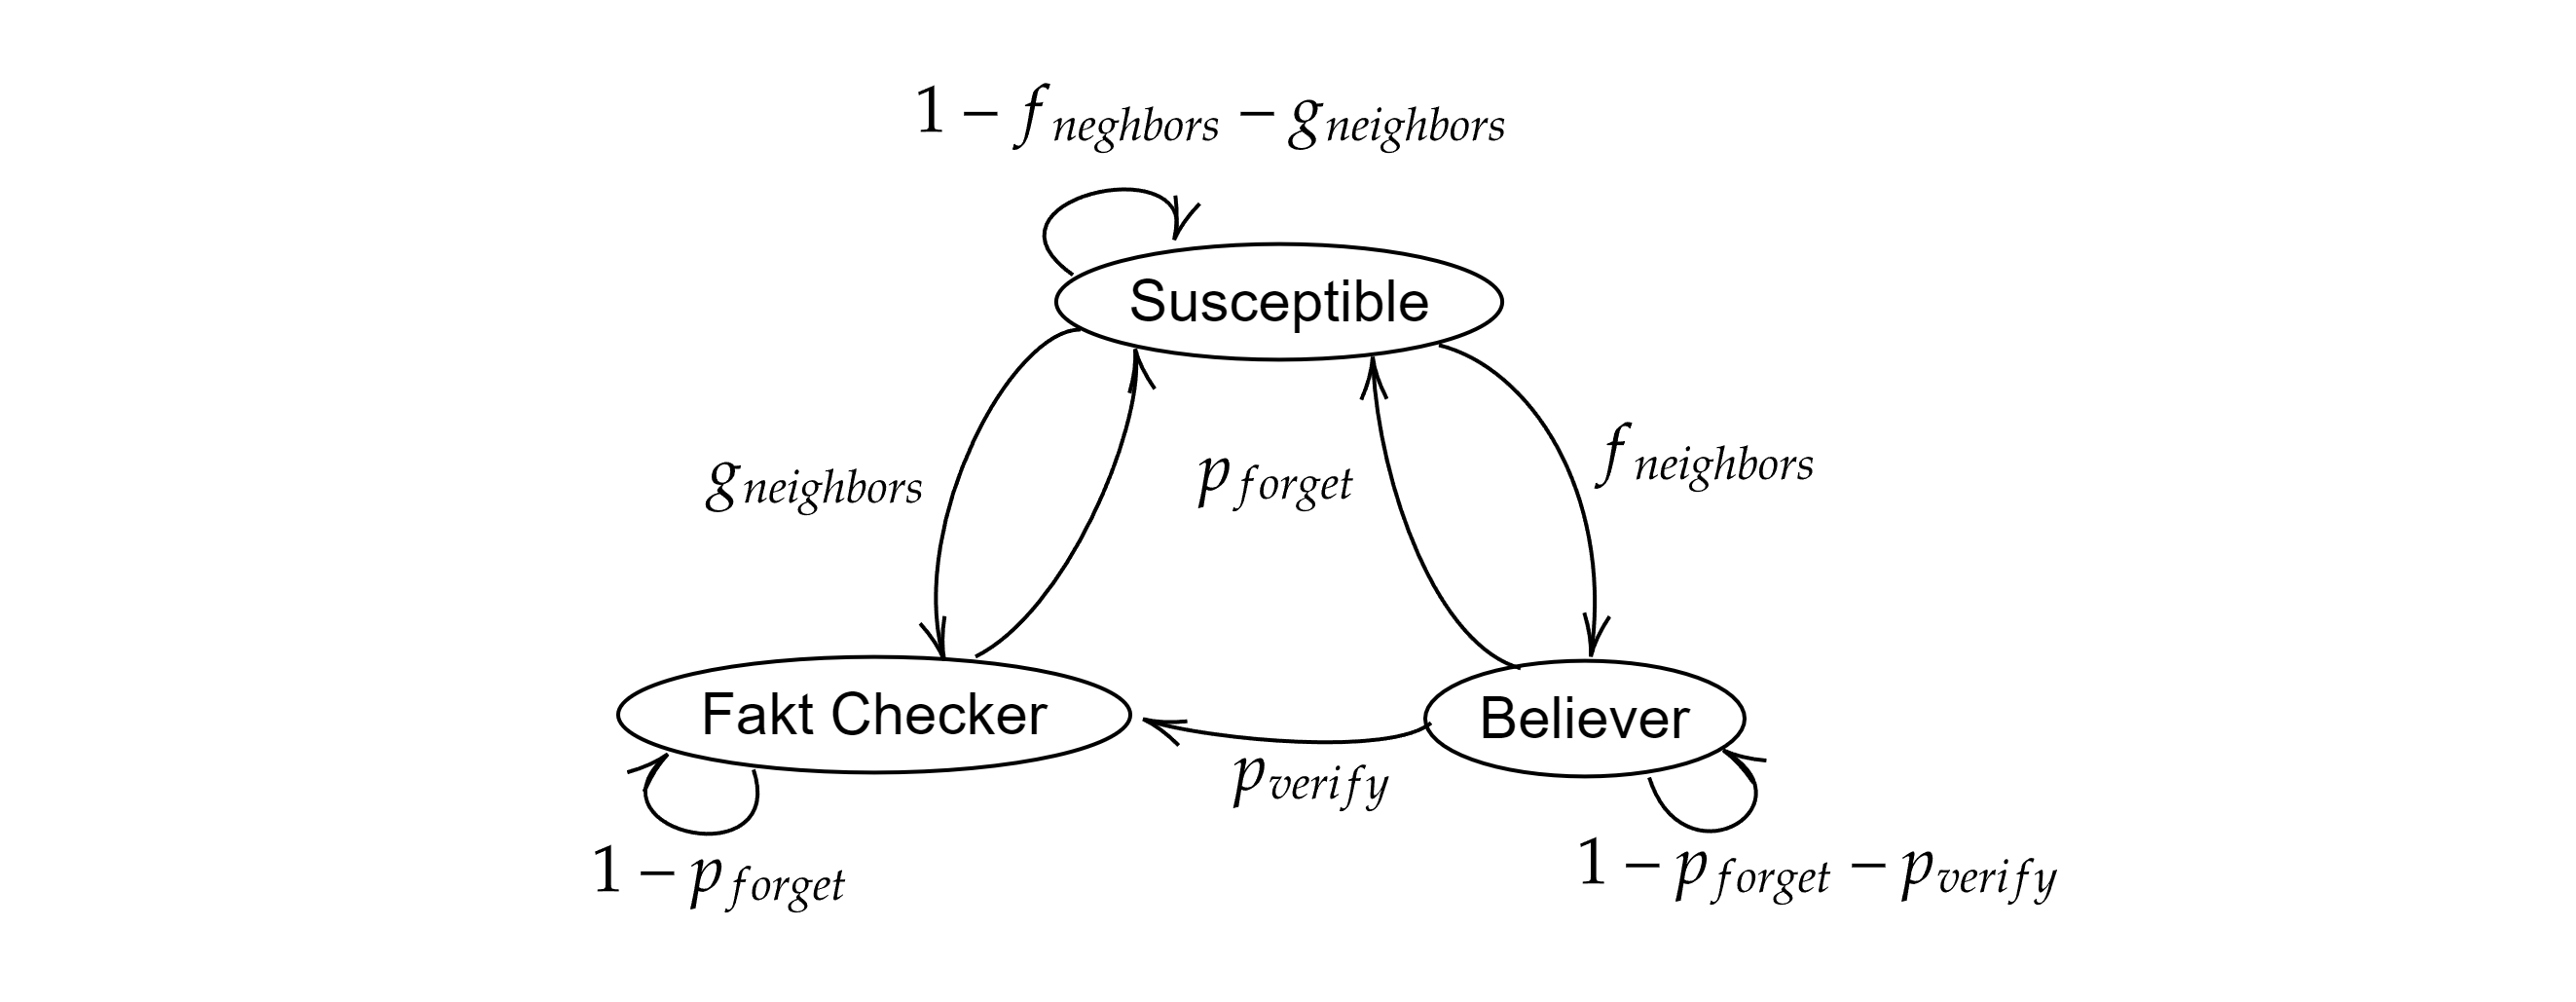
\includegraphics[scale=.9]{figs/Tambuscio.png}
    \caption{State chart for the model \cite{sirsmodel}}
    \label{originalmodelstatechart}
\end{figure}

\begin{table}[ht!]
    \centering
    \begin{tabular}{|c | c |} 
     \hline
     & \\
     $\begin{aligned}
          p_i^S(t+1) &= p_{forget}(s_i^I(t)+s_i^R(t)) + (1-f_i-g_i)s_i^S(t) \\
          p_i^I(t+1) &= f_is_i^S(t) + (1-p_{forget}-p_{verify})s_i^I(t) \\
          p_i^R(t+1) &= g_is_i^S(t) + p_{verify}s_i^I(t)+(1-p_{forget})s_i^R(t)
        \end{aligned}$
      &
      $\begin{aligned}
          f_i(t) &= \beta \frac{n_i^I(t)(1+\alpha)}{n_i^I(t)(1+\alpha)+n_i^R(t)(1-\alpha)} \\
          g_i(t) &= \beta \frac{n_i^R(t)(1-\alpha)}{n_i^I(t)(1+\alpha)+n_i^R(t)(1-\alpha)} \\
        \end{aligned}$
       \\ 
       & \\
     \hline
    \end{tabular}
    \caption{Probability functions for the states \cite{sirsmodel}}
    \label{SIS-table-equations}
\end{table}

In Figure \ref{originalmodelstatechart}, the states and the general 
probabilities for transitions of the model are shown.
In Table \ref{SIS-table-equations}, the probability functions 
$p_i^S, p_i^I, p_i^R$ that a node $i$ will belong to each state  
\textit{Susceptible} ($S$),  \textit{Infected} ($I$) and 
\textit{Recovered} ($R$) at the iteration step $t+1$ are defined. 
These probability functions 
depend on the current state of the node $s_i=[s_i^S,  s_i^I,  s_i^R]$,
where $s_i^K$ is $1$ if the node $i$ has the state $K$ and else $0$.
Furthermore, the probability functions also depend on the constant system 
probabilities $p_{\mathrm{verify}}, p_{\mathrm{forget}}$. Last, the functions are also 
dependent on the propagation functions $f_i, g_i$, where $g_i$ describes 
the propagation of the fake news and $f_i$ the propagation of its debunking
for the node $i$. The two functions  $f_i, g_i$ are dependent on
the amount of neighbors $n_i^I, n_i^R$ that belong to the states
\textit{Infected} or \textit{Recovered} and the two 
system parameters $\beta$ and $\alpha$, where $\beta$ is the transmission rate
and $\alpha$ defines the credibility of the hoax. Thus, with this model it
is possible to model both the fake news spreading process and 
the fact-checking propagation process at the same time. 
Moreover, it is possible to consider the plausibility of the fake 
news in the propagation process.

Graph-based epidemological models view the infection process on an entity-level.
Thus, the state of each node in the system is always known.
However, another way to view epidemological models is by ignoring the 
state of each node and only calculating the number of nodes in each state.
As a consequence, this can be considered a system-level view.
This view can be modeled with differential equations.
For differential equations, the amount of entities belonging to each state may change 
after a time duration $\Delta t$. The equations to calculate the 
changes in number of entities in each state, and thus the progress 
of the information diffusion, can be seen in Table \ref{SI-table-equations}.
$\beta$ and $\gamma$ are the transition rate parameters of the model,
where $\beta$ is the transmission rate and $\gamma$ the 
recovery rate.

\begin{table}[ht!]
    \centering
    \begin{tabular}{|c | c |} 
     \hline
     SIR & SIS  \\ 
     \hline
     & \\
     $\begin{aligned}
          \frac{dS}{dt} &= -\beta I S \\
          \frac{dI}{dt} &= \beta I S - \gamma I \\
          \frac{dR}{dt} &= \gamma I  
        \end{aligned}$
      &
      $\begin{aligned}
          \frac{dS}{dt} &= -\beta I S + \gamma I\\
          \frac{dI}{dt} &= \beta I S - \gamma I
        \end{aligned}$
       \\ 
       & \\
     \hline
    \end{tabular}
    \caption{Model equations for SIR and SIS model \cite{sirequation}}
    \label{SI-table-equations}
\end{table}


\subsection{Information Cascade Models}

Another way to model information diffusion in graphs is by viewing the diffusion as a 
sequential information propagation process. That forms the foundational 
assumption within information cascade models. In this model 
\cite{reviewinformationdiffusion}, any node $n$ which is infected in the
iteration step $i$ may infect its connected neighbor $a$ with a 
probability $P_n(a)$. All nodes infected by node $n$
can then infect their neighboring node in the next iteration step $i+1$
and node $n$ becomes inactive and does not infect any neighbors in future
iterations.
Equation \ref{eqbasicpropagationcascading} 
shows how the propagation step is modeled.
Information cascade models are mostly used for prediction and influence 
analysis purposes, and not to explain the collective behavior
of the system during the information diffusion process.

\begin{equation}
    I(a) = 1 (\sum\limits_{\substack{(b,a)\in E, \\ b \in V \cap I}}
    1(f^{rand}\geq P_n(a))>0) 
    \label{eqbasicpropagationcascading}
\end{equation}

There are different subtypes of cascading models.
Some subtypes are described in \cite{diffusionbasics}. These are:

\begin{itemize}
    \item Independent Cascading Model: In this type of model, the 
    probability $P_n(a)=p$ is constant for each node $a$ and neighbor $n$.
    Thus, the probability function does not depend on the history 
    of the system and its information diffusion status.
    \item Decreasing Cascading Model: In this type of model, the probability
    function to activate the node $a$ decreases with each attempt of its 
    neighbors. This means that if a neighbor $n$ unsuccessfully tries to infect
    $a$ at iteration step $i$, then the probability that the neighbor $m$
    can sucessfully infect $a$ at step $i+t$ is lower.
\end{itemize}

\subsection{Threshold Models}
An additional method to analyze the diffusion process in graphs is by viewing the
propagation step as a process where each entity needs to overcome a 
specific threshold $\theta$ to become infected. More specifically, 
a certain number of neighbors need to be infected for node $a$ to become 
infected. Contrary to cascade models, a node can always 
infect its neighbors as long as the conditions are fulfilled in the threshold 
model. Equation \ref{eq:threshold} shows the general definition 
for the threshold model.

\begin{equation}
    I(a) = \sum\limits_{\substack{(b,a)\in E, \\ b \in V \cap I}}
    1 > \theta    
    \label{eq:threshold}
\end{equation}

Subtypes of this kind of diffusion model differ by the threshold parameter.
Some subtypes described in \cite{diffusionbasics} are:

\begin{itemize}
    \item Majority Threshold Model: A node $a$ becomes
    infected if the majority of its neighbors are infected, thus 
    $\theta = \frac{1}{2}c_a$.
    \item Small Threshold Model: The threshold for which
    node $a$ becomes infected is very small. The advantage of this model is that 
    certain algorithms may be calculated faster \cite{diffusionbasics}.
    \item Unanimous Threshold Model: All neighbors 
    of a node $a$ need to be infected for $a$ to become infected, thus
    $\theta = c_a$.
\end{itemize}


\section{Power Load Forecasting Methods}
\label{powerloadsection}

An important task in modern power grid management 
is to forecast power demand, so that the power supply can be adjusted accordingly.
The power demand forecasting methods can be categorized in three types:
short-, medium and long-term power demand forecast. These differ in which
timespan they forecast power demand. Most forecasting models are 
either statistical models or artifical intelligence based models 
\cite{raza2015review}. For these models to be able to predict the power 
demand, they need input data which correlate with the power 
usage. 

\subsection{Variables used for Power Load Forecasting}
\label{variabledependency}
Variables that correlate with power load 
can be classified as either endogenous or exogenous variables.
Exogenous variables can be considered as independent variables 
whose values are determined outside of the system. 
Endogenous variables, on the other side, 
are variables that are dependent of other variables in the 
model.

In the context of power load prediction, the most commonly 
used endogenous variable is the historical power load data.
For exogenous variables, there are multiple types of 
variables that are often considered as possible input data.
The first type of variables are \textit{environmental} variables like temperature, 
rainfall, humidity or wind power. A different type of variables are \textit{time} data
such as the specific weekday, if a day is a holiday and the time of the day.
Another type of variables are \textit{socio-economic} variables such as the
population size and growth, the exchange rate, the income level,
the gross domestic product or the different types and amount 
of consumers like agricultural, industrial or household consumers.
The last type of variables are \textit{building and occupancy related} variables such
as the household appliance usage,
the number of persons or the number of bedrooms in a household.

The relevance of each type of variables depend on if the model is
a short-, middle- or long-term power load forecasting model. For 
long-term predictions, the more slowly changing variables such as socio-economic
variables become more important than short-term variables such as weather data 
\cite{loadforecastingtimedependency2}\cite{loadforecastingtimedependency}.
The specific task definition is also relevant for the parameter selection.
Power load prediction models for residential buildings may benefit from 
building and occupancy related variables, but for a prediction model on a 
macroeconomic scale, socio-economic variables are more important.

Exogenous variables that are explicitly linked to human behaviour, 
such as social media usage, traffic information, satellite image data or 
internet usage, are not used often for power load forecasting. 
But these are the variables that would probably be affected in a change of 
human behavior. Therefore, these variables are analyzed for this Thesis.

Social media data does not directly correlate with power demand, but it is
possible to extract information relevant for power demand forecasting
from the content generated by it.
First, it is possible to analyze the spatial density of people by 
counting the amount of tweets tagged in a specific location of interest. 
It was shown that there is a significant
correlation between the number of geotagged tweets
and the power consumption in a specific region \cite{twittergeoloccorr}.
As a possible explanation for this correlation is that 
increased human activity in a specific region leads to a greater 
use of facilities such as heating or air conditioning in buildings or 
other types of power-consuming behavior.
For this reason, geotagged tweets were used as input data for 
power load forecasting models 
\cite{twittergeolocforecasting} \cite{twittergeolocforecasting2}.
Second, it is also possible to analyze the content written in the 
social media posts. The content in social media posts can be 
analyzed in two ways: 
It can either be analyzed by searching for posts with a defined keyword or tag
or it can be analyzed by using natural language processing techniques. 
In natural language processing, the raw text content 
(and possibly its metadata and attachements) of a post is analyzed
to extract the desired information. Possible analysis
methods would be to classify if a post is related to some energy-consuming
behavior or to count the number of keywords related to energy usage in the text.
For example, a natural language processing model was trained to 
classify specifically energy-related tweets \cite{energybert}.
The other possibility is to query the social media instance 
to find all posts that contain a specific keyword or tag.
This method is usually simpler than using more sophisticated natural 
language processing techniques, but increases the number of false positive 
posts that are not relevant for the specific task.
For power load prediction tasks, usually only the keyword search method is used.
In the work of \textit{LaLone et al.}, they show that the number of energy
related tweets during hurricane Katrina correlated with the number of 
power outages at the same time \cite{poweroutagetwitter}.
Another work uses twitter data with both keyword search and 
tweets that were classified with natural language processing techniques to
to find power outage regions \cite{twitterpoweroutagelighttime}.
In addition, another work used topic mining techniques to find
events on twitter posts that correlate with energy consumption 
\cite{twittertopicevent}.
Search engine indices are also a data type that can be considered 
as partially related to social network data, since it shows the 
interest that greater parts of the population have for a specific topic.
In the work of \textit{Wu et al.}, it was proven that adding 
keyword search counts can improve power load forecasting accuracy 
\cite{googlepowerforecast}.

General internet traffic data also correlates with power usage.
\textit{Morleya et al.} concludes that 
electricity consumed by information and communication devices
may contribute to increased peak electricity demand 
\cite{internettrafficenergycorrelation}.
Therefore, internet traffic data can be used as input data for 
power demand forecasting models \cite{electricityinternetforecast}. 

Studies show that with the increased adoption of electric vehicles (EV), 
there is an increased interdependency between the electric and 
transportation infrastructure \cite{interdependnytrafficenergy}. 
Traffic data may correlate with power load in two ways:
First, with traffic movement patterns, it is possible to follow the
movement patterns of larger groups of people. As an example, in the morning,
traffic intensity increases since a larger part of the population needs
to go to their workplace. Subsequently, this population group
returns back to their residences after finishing their work in the afternoon.
Thus, there is also an increased traffic intensity in the afternoon.
This traffic movement can be analyzed by measuring the 
incoming and outgoing traffic volume at the main roads of the 
region of interest. The usage of this variable in power load
forecasting models gained more interest during the COVID-19 pandemic, 
where drastically changing mobility and power consumption 
patterns meant that new model inputs were necessary to consider changing
behavior patterns in the population 
\cite{covidtrafficpower} \cite{covidtrafficpower2}.
But traffic data also correlated with the electricity consumption pattern
before the pandemic. One work showed that
using traffic data as an input for power load
forecasting models leads to more accurate predictions, even before
the COVID-19 pandemic \cite{causalmodeltrafficelectricity}.
Second, with the increasing EV usage in the future, 
the total power demand increases since these types of vehicles 
need to be charged. Power load forecasting methods that consider this
issue often focus on charging stations \cite{evcharchingstations}
\cite{evcharchingstations2}. However, changes in household power consumption 
and the general charging behavior of households
were also the objective of some studies. \textit{Gerossier et al.}
analyzed the different charging patterns in households
and found four different charging patters in which its members charged at 
a similar time and duration \cite{gerossier2019modeling}.
In addition, there are also works that describe
power load prediction models for individual household
charging forecasts \cite{skala2023interval}. 
A notable work was done by \textit{Arias et al.} that also considered 
traffic patterns
and analyzed the differences in EV charging behaviors between
commercial and residential districts for power demand forecasting
\cite{arias2016electric}.

The last variable that depends on human behavior mentioned in this Section are
satellite images. This type of images can be used to find a variety 
of enviromental factors relevant for power demand.
Satellite images are mostly used to forecast power generation of 
renewable resources such as solar power \cite{solarprediction}.
However, it can also be used to estimate household power consumption,
especially during nighttime. This is particularly of relevance for regions 
where the electricity consumption data is unreliable, such as in developing contries
\cite{reviewnighttime}. There is a correlation 
between nighttime light intensity and power consumption.
But this relation depends on the type of consumer, e.g. households or industry. 
Furthermore, the relation is not linear \cite{nighttimepowerestimation}. 
An issue when using nighttime images for power demand prediction is 
the inherent noise in the data. Non-household light sources such as 
streetlights and vehicles add noise to the images \cite{reviewnighttime}.
Another application of nighttime satellite image is for power outage detection.
If there is a power outage, the affected region will turn dark, which 
can be detected in satellite images. Satellite image data 
was successfully used in multiple power outage detection models
\cite{nightpoweroutage} \cite{twitterpoweroutagelighttime}.

\subsection{Load Profiles as Power Load Forecasting Models}
\label{loadprofilebasic}
Another method to estimate the power demand for a specific time are load 
profiles. Load profiles describe representative power usage patterns 
of costumers over time. Load profiles are 
representative load curves and thus are independent of input variables.
Load profiles differ by the type of custormer they represent. For 
example, the load profiles provided by the German Federal Association of 
Energy and Water Management (Bundesverband der Energie- und Wasserwirtschaft 
e. V. (BDEW)) can be divided by households, commerce, 
farms, and other types of customers \cite{meier1999reprasentative}.
There are three methods to model load profiles.
Bottom-up models analyze the electricity consumption of individual customers
and extrapolate the findings to a group of customers, e.g. households.
For household customers, the appliance usage and electricity consumption 
and the behavior patterns of the inhabitants are analyzed to model
the power consumption. Top-down models use the total power consumption 
estimates to approximate the power consumption of individual consumers.
Hybrid models combine both bottom-up and top-down models to model 
load profiles. 


\chapter{Related Works}

In light of the increasing usage of web-based technologies in our daily 
lifes, web-based points of attacks that could attack a country's 
electrical infrastructure and other critical infrastructure 
are becoming an increasing concern.
Thus, the resilience of the electrical grid is in danger.

%One of these points of attack created by web-based technologies
%are direct attacks via cyber attacks. The increased usage of 
%smart grids, which uses the internet to support a variety of functions 
%to make the electrical grid more efficient, increases the 
%vulnerability of the electrical grid to cyberattacks.
%Thus, cyber security for smart grids is a widely researched subject.
%The threat of cyberattacks are research from multiple angles.
%First, general vulnerabilities of the smart grid and the threats 
%created by possible cyberattacks can be analysed and discussed 
%\cite{cyberbasic1} \cite{cyberbasci2}.
%Second, the detection of cyber attacks on the electrical grids are 
%a wide resarch field. 

%Hier könnte man auch false pricing attack power grid als keyword noch
%weitersuchen
The point of attack relevant for this thesis are social network-based
attacks. These attacks try to influence the behavior of groups of people to 
change the electricity consumption on a scale that may threaten the reliability
of the electrical grid. This type of attack is not as well researched 
compared to cybersecurity-based attack points. All works in this topic
mainly consider false pricing attacks, where consumers receive false 
electricity pricing information over social media and change their 
electricity demand pattern because of the false information.
In the work of \textit{Tang et al.}, they model such kind of attack on the 
smart grid with a complex information propagation algorithm which considers 
multiple types of influences, consumers with different types of 
personalities and other characteristics \cite{falsepricing1}.
Furthermore, they analyse the possible reaction to the attack, where
the operators use load shedding to reduce the load on the energy system. 
Another work implements a model similar to the model
proposed by \textit{Tang et al.}, but with a focus on the consequences of a 
possible false pricing attack \cite{vulnerabilityanalysis}.

Another problem that can be analysed in this topic is which $k$ entities 
need to be influenced by misinformation to instill 
the maximum damage on the power grid. In the work of \textit{Pan et al.}, 
they analysed this issue, developing several heuristics to find the most 
relevant entities in the system that can inflict the maximum damage by both 
propagating the misinformation and increasing the demand 
$d_0$ to $d_0(1+\Delta i)$ \cite{pan2017threat}. 
Furthermore, they analysed load shedding as a
countermeasure for the targeted misinformation attack.
\textit{Nyugen et al.} extended the work of \textit{Pan et al.}
by further analysing the general vulnerability and also the resilience of 
the power grid if automatic load shedding is applied to the overloaded grid
\cite{nguyen2019vulnerability}.

A paper that tries to analyse a more practical development of a misinformation
attack is the paper of \textit{Raman et al.} \cite{raman2020weaponizing}.
In their work, they used a survey to analyse the probability of a person
reacting to misinformation, and thus increasing the electricity demand,
and how likely they are to forward the misinformation to other people.
Furthermore, they focused on possible impacts on the electrical grid in 
the future by also analysing the consequences of the increased 
usage of electric vehicles in the future. Possible countermeasures like
load shedding were not analysed.

Last, in the work of \textit{Jamalzadeh et al.}, they created a model to monitor
the power grid when its under a misinformation attack and to analyse
how a possible campaign to counter the misinformation attack can mitigate
the impacts of the attack \cite{jamalzadeh2022protecting}. Furthermore,
they describe an optimization algorithm to minimize the amount of 
entities affected by a possible blackout caused by the attack as 
a countermeasure mechanism.
\chapter{Implementation of the Simulation Framework to model the Effect
of Information on Social Media on the Power Grid}

In this chapter, the simulation framework that was implemented for this thesis
will be introduced.
First, the model for the social media network, which includes both the 
random graph generation and the information diffusion model, will be introduced
(Section \ref{socialmediasection}).

\section{Modelling of the Social Media Network}
\label{socialmediasection}





\chapter{Results}

The experiments outcome should be critically discussed. A conclusion about the theory based on the experiments follows. Failures and shortcomings of the theoretical model should be pointed out and explained as necessary.
\chapter{Conclusion}
\label{conclusion}

The COVID-19 pandemic showed that drastic changes in 
consumer behavior can lead to significant supply chain issues.
As a consequence, there is a growing interest in researching 
how shifts in demand manifest during crises. 
Critical infrastructure such as the power grid
do not seem to have been yet affected by such demand changes.
Nonetheless, these demand shifts could affect the critical 
infrastructure in the future. In order to 
formulate countermeasures to such risks, it is 
important to analyze how these demand shifts could 
arise and how they would progress. In this thesis,
a framework was implemented to simulate the effects of 
changes in consumer behavior. The focus was set on
consumer behavior changes based on the spread
of information on social media. 
The simulation framework was implemented using 
a Barabási–Albert random graph as a representation for social 
media networks. Moreover, an epidemological model, 
the susceptible-infectious-recovered model, is used to model 
the information propagation in a social media network.
In addition, an algorithm was implemented to estimate 
simulation parameters based on real social media 
data. 

The simulation framework was used to analyze both 
the simulation framework and the effects of information 
on social media on consumer behavior and 
consequently on the power grid infrastructure.
For this, four different 
scenarios were introduced where information
on the internet could lead to consumer demand changes. 
The first scenario dealt with the concept of 
demand-response programs. The second focused on 
coordinated acts by a conspiracy theorists to destabilize 
the power grid. The third one dealt with rumors leading 
to a mass panic, thus leading people to charge their 
electric vehicles and leaving their homes in masses.
The last one comprises of an emergency message 
which requests people to shower immediately.
The analysis of the scenarios 
showed that syncronized consumer
demand changes pose a significant threat to the power
grid. The risk for the power grid depends on the percentage
of the population that is willing to change their behavior 
due to the information being spread.
Furthermore, the adoption
of energy-intensive technologies such as 
electric vehicles may increase the 
effects of syncronized consumer demand changes
on the infrastructure. 
Hence, the risk of excess power demand events may
elevate with increased adoption of new, energy consuming 
technologies in society.
The results show that policymakers should consider the
threat of misinformaion and formulate countermeasures
to deal with possible consequences of such events.

\section{Future Works}

The work described in this thesis can be extended in multiple
directions. First, more scenarios could be researched 
to analyze the effects of changes in consumer behavior
on the power grid further. Second, more real world 
data sources could be used in conjunction with the 
simulation framework.
In Section \ref{variabledependency}, different data 
sources were introduced and their relevance in regards 
to power load forecasting were explained. For this
thesis, only social media data was used to estimate system 
parameters. However, other data sources could be used
to either estimate simulation parameters or to predict
sudden changes in consumer demand. For example,
traffic data could be used to analyze movement flows 
between different parts of a city. Therefore, the
traffic flow out of residential districts into 
commercial and industrial districts of the city 
could be observed. With this,
the percentage of households with at least one 
resident at home could be estimated. 
This would allow for a more realistic estimation 
of which households could affect the power grid.
Third, the excess power consumption could be mapped
to a physical location. Consequently, with this, 
the power demand changes could be mapped to the 
physical power grid infrastructure. Thus, 
critical levels of demand changes can be 
checked with the local critical thresholds of the
local power grid connections. Social media data could
be used to estimate the possible location of the 
posting entities \cite{jurgens2015geolocation}.
However, other possible methods could be analyzed.
Forth, more detailed methods to estimate excess 
power consumption could be analyzed.
In Section \ref{loadprofilebasic}, the concept 
of load profiles were introduced. One 
method to generate load profiles is by 
creating a model which 
analyzes the power consumption of a single 
household and extrapolates the results to 
a group of households. The model includes 
the appliance usage in a household. 
Those models could be used to create more 
realistic excess power consumption data
by dynamically activating and deactivating
household appliances of the model when 
households are considered as 
\textit{Infected} in the SIR model.
Fifth, the process of gathering relevant social 
media posts could be analyzed. In this thesis,
it is assumed that the relevant social 
media posts are already known. However,
finding posts that are of importance for 
specific scenarios may be difficult and 
dependent on which specific scenario is 
occuring. Thus, further work in analyzing 
how to gather relevant posts is necessary.
Sixth, possible countermeasures for this type 
of risk could be proposed. In other related works,
load shedding was introduced as a method to 
deal with misinformation-based attacks on the power grid.
However, other possible countermeasures to deal with 
this kind of danger could be considered.



%\appendix

%\input{inc/diaApx.tex}


		
\printbibliography
\chapter{Appendix}

\begin{lstlisting}[language=json,firstnumber=1, 
    caption={Configuration file for scenario 1
    },captionpos=b,label={scenario1config}]
{
    ...
    "model_args":{
        "electric_car": {
        "power": 1125,
        "p": 0.1,
        "duration": 10000
        },
        "washing_machine": {
        "power": 100,
        "p": 95.8,
        "duration": 4
        },
        "dishwasher": {
        "power": 300,
        "p": 71.7,
        "duration": 8
        } 
    },
    "sim": {
        "p_will_act": 0.6,
        "power_usage": 0.8,
        "p_verify": 0.07,
        "alpha": 0.4,
        "beta": 0.6,
        "power_threshold": 1.5
        "factor": 1
    },
    "network":{
        "nodes": 400
      }, 
}
\end{lstlisting}
\end{document}
